\section{Planificación Gantt}

\par Utilizando la herramienta Microsoft Project, hemos realizado el diagrama de Gantt, mostrando tanto la planificación como el seguimiento del proyecto semana a semana. El proyecto para CARSAFETY constará de 12 hitos:

\begin{enumerate}
  \item Fin fase de documentación
  \item Fin de la planificación
  \item Fin análisis de la primera iteración
  \item Fin diseño de la primera iteración
  \item Fin de la primera iteración
  \item Fin análisis de la segunda iteración
  \item Fin diseño de la segunda iteración
  \item Fin de la segunda iteración
  \item Fin análisis de la tercera iteración
  \item Fin diseño de la tercera iteración
  \item Fin de la tercera iteración
  \item Fin del proyecto
\end{enumerate}
\clearpage

\par A continuación se muestra la planificación que se ha llevado a cabo. Los acrónimos utilizados en la especificación de los recursos para cada tarea son los siguientes:
\begin{itemize}
  \item AG: Alberto García Hernández.
  \item DG: Daniel González de la Hera.
  \item JA: Juan Abascal Sánchez.
  \item CO: Carlos Olivares Sánchez-Manjavacas.
  \item CT: Carlos Tormo Sánchez.
  \item AL: Adriana Lima.
  \item IS: Irina Shayk. 
\end{itemize}

\begin{center}
\begin{longtable}{  p{0.5cm}  p{1cm}  p{2cm}  p{4cm}  p{1.5cm}  p{2cm}  p{2cm}  p{2cm}  }

  %HEAD
  \textbf{Id} & \textbf{Número}  & \textbf{Recursos} & \textbf{Nombre de tarea} & \textbf{Duración} & \textbf{Comienzo} & \textbf{Fin} & \textbf{Predecesor}  \\ \hline \hline
  \endfirsthead
  \textbf{Id} & \textbf{Número}  & \textbf{Recursos} & \textbf{Nombre de tarea} & \textbf{Duración} & \textbf{Comienzo} & \textbf{Fin} & \textbf{Predecesor}  \\ \hline \hline
  \endhead

  %FOOT
  \multicolumn{7}{r}{\textit{Continúa en la siguiente pagina}} \\
  \endfoot
  \endlastfoot

	%TABLE
  1	&	1	&	AG, DG, JA, AL	&	Fase de Documentación	&	23 días	&	mié 01/02/17	&	vie 03/03/17	&		\\ \hline
2	&	1.1	&	AG, DG	&	   Oferta y Documento de Control de Costes	&	3 días	&	mié 01/02/17	&	vie 03/02/17	&		\\ \hline
3	&	1.2	&	AG, DG	&	   Estudio de la Viabilidad del Sistema	&	10 días	&	lun 06/02/17	&	vie 17/02/17	&	2	\\ \hline
4	&	1.3	&	AG, AL	&	   Plan de Gestión de la Calidad	&	5 días	&	lun 20/02/17	&	vie 24/02/17	&	3	\\ \hline
5	&	1.4	&	AG, JA	&	   Plan de Gestión de la Configuración 	&	5 días	&	lun 27/02/17	&	vie 03/03/17	&	4	\\ \hline
6	&	1.5	&	AG	&	   Fin de la fase de Documentación	&	0 días	&	vie 03/03/17	&	vie 03/03/17	&		\\ \hline
7	&	2	&	AG, DG, JA	&	Planificación y Especificación de Requisitos	&	7 días	&	lun 06/03/17	&	mar 14/03/17	&		\\ \hline
8	&	2.1	&	AG, DG, JA	&	   Diagrama de Casos de Uso	&	4 días	&	lun 06/03/17	&	jue 09/03/17	&		\\ \hline
9	&	2.2	&	DG, JA	&	   Descripción de Casos de Uso de Alto Nivel	&	3 días	&	vie 10/03/17	&	mar 14/03/17	&	8	\\ \hline
10	&	2.3	&	AG, DG	&	   Estimación y Priorización	&	3 días	&	vie 10/03/17	&	mar 14/03/17	&	8	\\ \hline
11	&	2.4	&	AG	&	   Fin de la Planificación	&	0 días	&	mar 14/03/17	&	mar 14/03/17	&		\\ \hline
12	&	3	&		&	Construcción	&	130 días	&	mié 15/03/17	&	mié 13/09/17	&		\\ \hline
13	&	3.1	&	AG, DG, JA, AL, CT, IS, CO	&	   Primera Iteración	&	43 días	&	mié 15/03/17	&	vie 12/05/17	&		\\ \hline
14	&	3.1.1	&	AG, DG, JA, AL	&	      Análisis	&	8 días	&	mié 15/03/17	&	vie 24/03/17	&		\\ \hline
15	&	3.1.1.1	&	DG	&	         Casos de Uso Expandidos	&	2 días	&	mié 15/03/17	&	jue 16/03/17	&	11	\\ \hline
16	&	3.1.1.2	&	JA, AL	&	         Contrato de Operaciones	&	2 días	&	vie 17/03/17	&	lun 20/03/17	&	15	\\ \hline
17	&	3.1.1.3	&	DG, JA	&	         Modelo Conceptual	&	2 días	&	mar 21/03/17	&	mié 22/03/17	&	16	\\ \hline
18	&	3.1.1.4	&	AG, DG	&	         Arquitectura de Sistema	&	2 días	&	jue 23/03/17	&	vie 24/03/17	&	17	\\ \hline
19	&	3.1.1.5	&	AG	&	         Fin de Análisis	&	0 días	&	vie 24/03/17	&	vie 24/03/17	&		\\ \hline
20	&	3.1.2	&	AG, DG, AL, JA	&	      Diseño	&	4 días	&	lun 27/03/17	&	jue 30/03/17	&		\\ \hline
21	&	3.1.2.1	&	DG, AL	&	         Diagrama de Clases	&	2 días	&	lun 27/03/17	&	mar 28/03/17	&	19	\\ \hline
22	&	3.1.2.2	&	AG, DG, AL	&	         Diagrama de Transición de Estados	&	2 días	&	lun 27/03/17	&	mar 28/03/17	&		\\ \hline
23	&	3.1.2.3	&	AG, AL, JA	&	         Diagrama de Secuencia	&	2 días	&	mié 29/03/17	&	jue 30/03/17	&	21	\\ \hline
24	&	3.1.2.4	&	AG	&	         Fin Diseño	&	0 días	&	jue 30/03/17	&	jue 30/03/17	&		\\ \hline
25	&	3.1.3	&	DG	&	      Refinamiento del Plan	&	1 día?	&	jue 30/03/17	&	jue 30/03/17	&	24	\\ \hline
26	&	3.1.4	&	DG	&	      Sincronización de Modelos	&	1 día?	&	vie 31/03/17	&	vie 31/03/17	&	25	\\ \hline
27	&	3.1.5	&	CT, IS	&	      Desarrollo	&	30 días	&	lun 03/04/17	&	vie 12/05/17	&	26	\\ \hline
28	&	3.1.6	&	CO	&	      Pruebas	&	25 días	&	lun 10/04/17	&	vie 12/05/17	&	26	\\ \hline
29	&	3.1.7	&	AG	&	      Fin de la Primera Iteración	&	0 días	&	vie 12/05/17	&	vie 12/05/17	&		\\ \hline
30	&	3.2	&	AG, DG, JA, AL, CT, IS, CO	&	   Segunda Iteración	&	43 días	&	vie 12/05/17	&	mar 11/07/17	&		\\ \hline
31	&	3.2.1	&	AG, DG, JA, AL	&	      Análisis	&	9 días	&	vie 12/05/17	&	mié 24/05/17	&		\\ \hline
32	&	3.2.1.1	&	DG	&	         Casos de Uso Expandidos	&	2 días	&	vie 12/05/17	&	lun 15/05/17	&	29	\\ \hline
33	&	3.2.1.2	&	JA, AL	&	         Contrato de Operaciones	&	2 días	&	mié 17/05/17	&	jue 18/05/17	&	32	\\ \hline
34	&	3.2.1.3	&	DG, JA	&	         Modelo Conceptual	&	2 días	&	vie 19/05/17	&	lun 22/05/17	&	33	\\ \hline
35	&	3.2.1.4	&	AG, DG	&	         Arquitectura de Sistema	&	2 días	&	mar 23/05/17	&	mié 24/05/17	&	34	\\ \hline
36	&	3.2.1.5	&	AG	&	         Fin de Análisis	&	0 días	&	mié 24/05/17	&	mié 24/05/17	&		\\ \hline
37	&	3.2.2	&	AG, DG, AL, JA	&	      Diseño	&	5 días	&	mié 24/05/17	&	mar 30/05/17	&		\\ \hline
38	&	3.2.2.1	&	DG, AL	&	         Diagrama de Clases	&	2 días	&	mié 24/05/17	&	jue 25/05/17	&	36	\\ \hline
39	&	3.2.2.2	&	AG, DG, AL	&	         Diagrama de Transición de Estados	&	2 días	&	jue 25/05/17	&	vie 26/05/17	&		\\ \hline
40	&	3.2.2.3	&	AG, AL, JA	&	         Diagrama de Secuencia	&	2 días	&	lun 29/05/17	&	mar 30/05/17	&	39	\\ \hline
41	&	3.2.2.4	&	AG	&	         Fin Diseño	&	0 días	&	mar 30/05/17	&	mar 30/05/17	&		\\ \hline
42	&	3.2.3	&	DG	&	      Refinamiento del Plan	&	1 día?	&	mar 30/05/17	&	mar 30/05/17	&	41	\\ \hline
43	&	3.2.4	&	DG	&	      Sincronización de Modelos	&	1 día?	&	mar 30/05/17	&	mar 30/05/17	&	41	\\ \hline
44	&	3.2.5	&	CT, IS	&	      Desarrollo	&	30 días	&	mié 31/05/17	&	mar 11/07/17	&	43	\\ \hline
45	&	3.2.6	&	CO	&	      Pruebas	&	25 días	&	mié 07/06/17	&	mar 11/07/17	&		\\ \hline
46	&	3.2.7	&	AG	&	      Fin de la Segunda Iteración	&	0 días	&	mar 11/07/17	&	mar 11/07/17	&		\\ \hline
47	&	3.3	&	AG, DG, JA, AL, CT, IS, CO	&	   Tercera Iteración	&	46 días	&	mar 11/07/17	&	mié 13/09/17	&		\\ \hline
48	&	3.3.1	&	AG, DG, JA, AL	&	      Análisis	&	9 días	&	mar 11/07/17	&	vie 21/07/17	&		\\ \hline
49	&	3.3.1.1	&	DG	&	         Casos de Uso Expandidos	&	2 días	&	mar 11/07/17	&	mié 12/07/17	&	46	\\ \hline
50	&	3.3.1.2	&	JA, AL	&	         Contrato de Operaciones	&	2 días	&	vie 14/07/17	&	lun 17/07/17	&	49	\\ \hline
51	&	3.3.1.3	&	DG, JA	&	         Modelo Conceptual	&	2 días	&	mar 18/07/17	&	mié 19/07/17	&	50	\\ \hline
52	&	3.3.1.4	&	AG, DG	&	         Arquitectura de Sistema	&	2 días	&	jue 20/07/17	&	vie 21/07/17	&	51	\\ \hline
53	&	3.3.1.5	&	AG	&	         Fin Análisis	&	0 días	&	vie 21/07/17	&	vie 21/07/17	&		\\ \hline
54	&	3.3.2	&	AG, DG, AL, JA	&	      Diseño	&	4 días	&	lun 24/07/17	&	jue 27/07/17	&		\\ \hline
55	&	3.3.2.1	&	DG, AL	&	         Diagrama de Clases	&	2 días	&	lun 24/07/17	&	mar 25/07/17	&	53	\\ \hline
56	&	3.3.2.2	&	AG, DG, AL	&	         Diagrama de Transición de Estados	&	2 días	&	lun 24/07/17	&	mar 25/07/17	&	53	\\ \hline
57	&	3.3.2.3	&	AG, AL, JA	&	         Diagrama de Secuencia	&	2 días	&	mié 26/07/17	&	jue 27/07/17	&	56	\\ \hline
58	&	3.3.2.4	&	AG	&	         Fin Diseño	&	0 días	&	jue 27/07/17	&	jue 27/07/17	&		\\ \hline
59	&	3.3.3	&	DG	&	      Refinamiento del Plan	&	1 día	&	jue 27/07/17	&	jue 27/07/17	&	58	\\ \hline
60	&	3.3.4	&	DG	&	      Sincronización de Modelos	&	1 día	&	jue 27/07/17	&	jue 27/07/17	&	58	\\ \hline
61	&	3.3.5	&	CT, IS	&	      Desarrollo	&	30 días	&	vie 28/07/17	&	jue 07/09/17	&	60	\\ \hline
62	&	3.3.6	&	CO	&	      Pruebas	&	25 días	&	vie 04/08/17	&	jue 07/09/17	&		\\ \hline
63	&	3.3.7	&	AG	&	      Fin de la Tercera Iteración	&	0 días	&	mié 13/09/17	&	mié 13/09/17	&		\\ \hline
64	&	4	&	AG, AL	&	Implantación	&	3 días	&	mié 13/09/17	&	vie 15/09/17	&		\\ \hline
65	&	4.1	&	AG, AL	&	   Impantación	&	3 días	&	mié 13/09/17	&	vie 15/09/17	&	63	\\ \hline
66	&	4.2	&	AG	&	   Fin del Proyecto	&	0 días	&	vie 15/09/17	&	vie 15/09/17	&		\\ \hline
  \caption{Tabla de la planificación Gantt}
  \label{tab:tablagantt}
\end{longtable}
\end{center}

\par A continuación se muestra el contenido de la tabla anterior en formato de gráficos:
%Figura
\begin{figure}[h]
\begin{center}
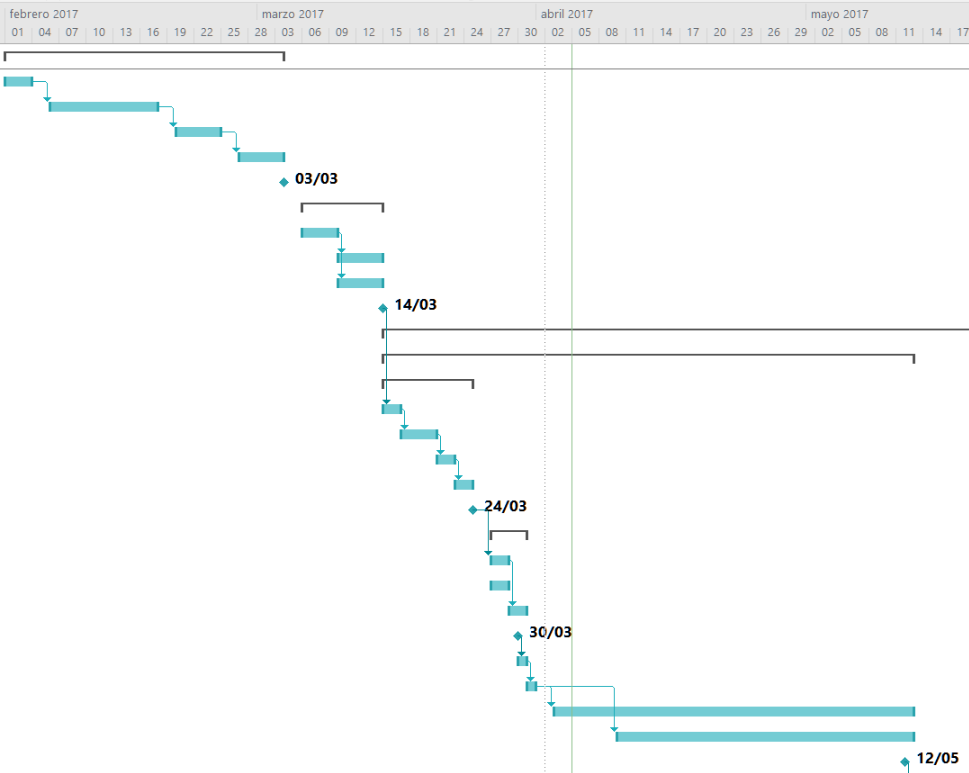
\includegraphics[width=0.6\textwidth]{./img/Gantt1.png}
\end{center}
\caption{Primer gráfico Gantt}
\label{tab:gantt1}
\end{figure}

%Figura
\begin{figure}[h]
\begin{center}
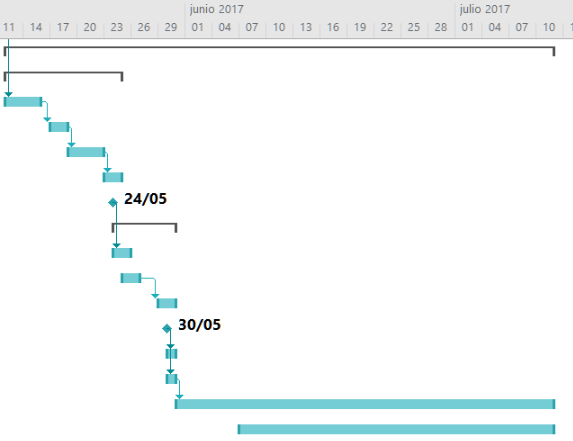
\includegraphics[width=0.6\textwidth]{./img/Gantt2.png}
\end{center}
\caption{Segundo gráfico Gantt}
\label{tab:gantt2}
\end{figure}

%Figura
\begin{figure}[H]
\begin{center}
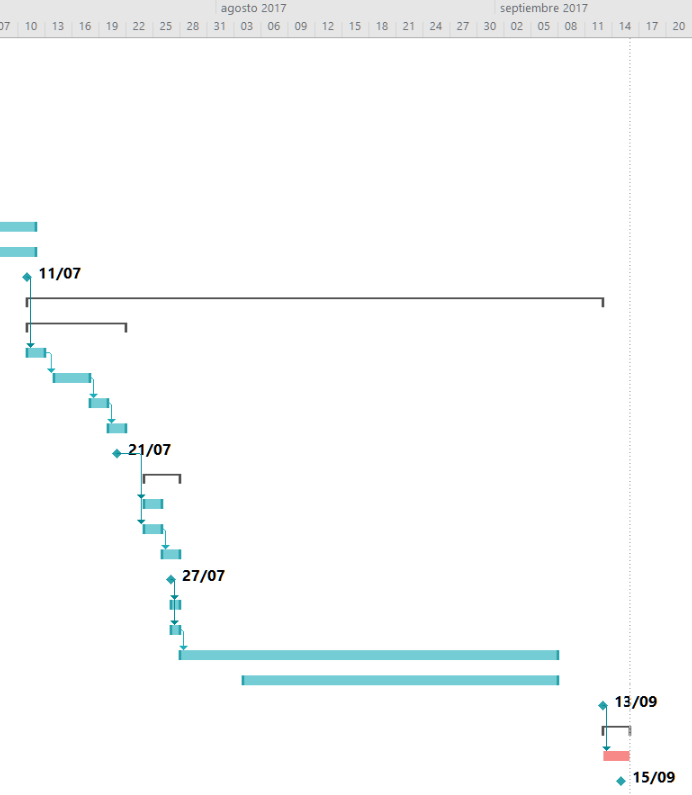
\includegraphics[width=0.6\textwidth]{./img/Gantt3.png}
\end{center}
\caption{Tercer gráfico Gantt}
\label{tab:gantt3}
\end{figure}
